\section{PARTIAL RESULTS}
    \subsection{Synthetic Dataset}
    Visually, the images generated by the Blender rendering are convincing for humans and may be used in future tasks of this project, reaching the main goal of this step. 
    The main concern about rendering synthetic images for this application is the photo-realism, given the main purpose of recognizing real entities in real world.
    With a reliable dataset of synthetic images and a unrendered 3D model for Blender, even without the CNN training in mind, applications in real time simulations is perfectly possible.
    
    The results showed promising behavior of the network with the synthetic bank in early stages without normalization of the amplitudes, as shown in Fig. \ref{fig:adagrad_orig}. 
    Later, batch normalization was applied with the approach described in \cite{BatchNormalization}, and the results were improved, as shown in Fig. \ref{fig:adam_norm} for the optimization with ADAM, and Fig. \ref{fig:adagrad_norm} for the otimization with ADAGRAD, with MSE = 0.0022 and RMSE = 0.0477 in the latter case.
    
        \begin{figure}[!h]
            \centering
            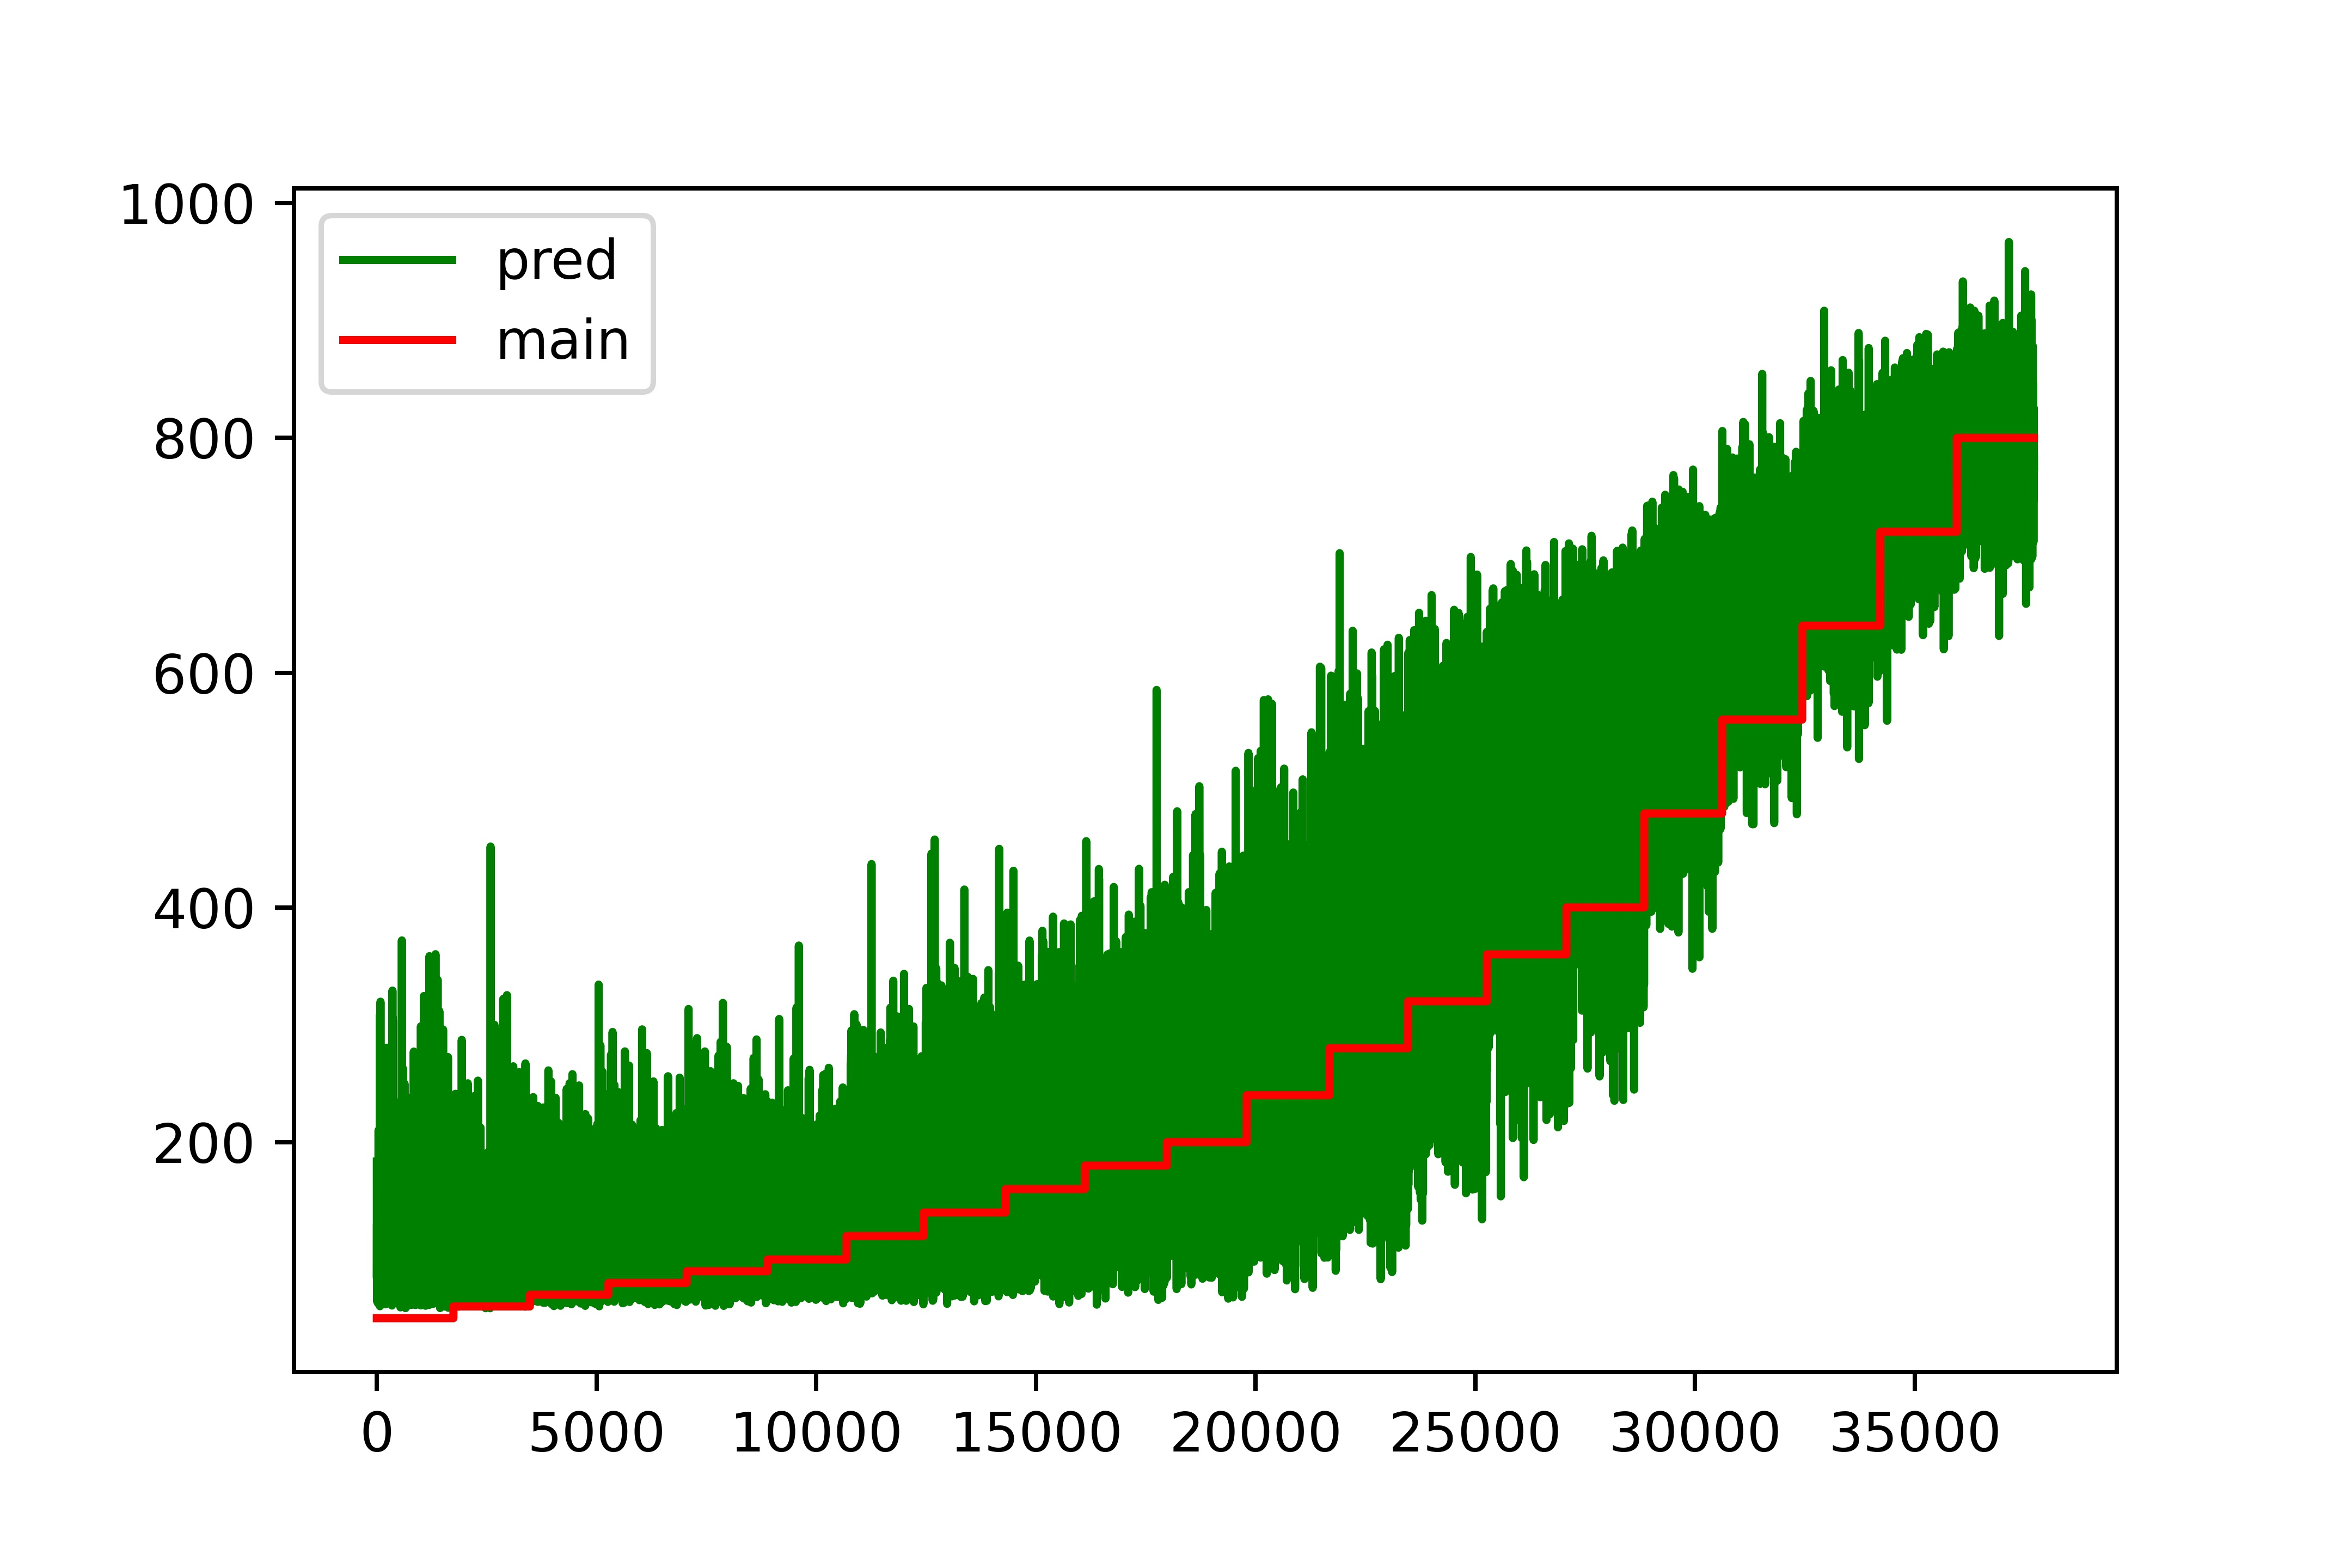
\includegraphics[width=12cm]{Images/plot_ada_orig.jpg}
            \caption{Initial result with ADAGRAD optimizer. In Green, the predictions output. In red, the real values.}
            \label{fig:adagrad_orig}
        \end{figure}
        
        \begin{figure}[!h]
            \centering
            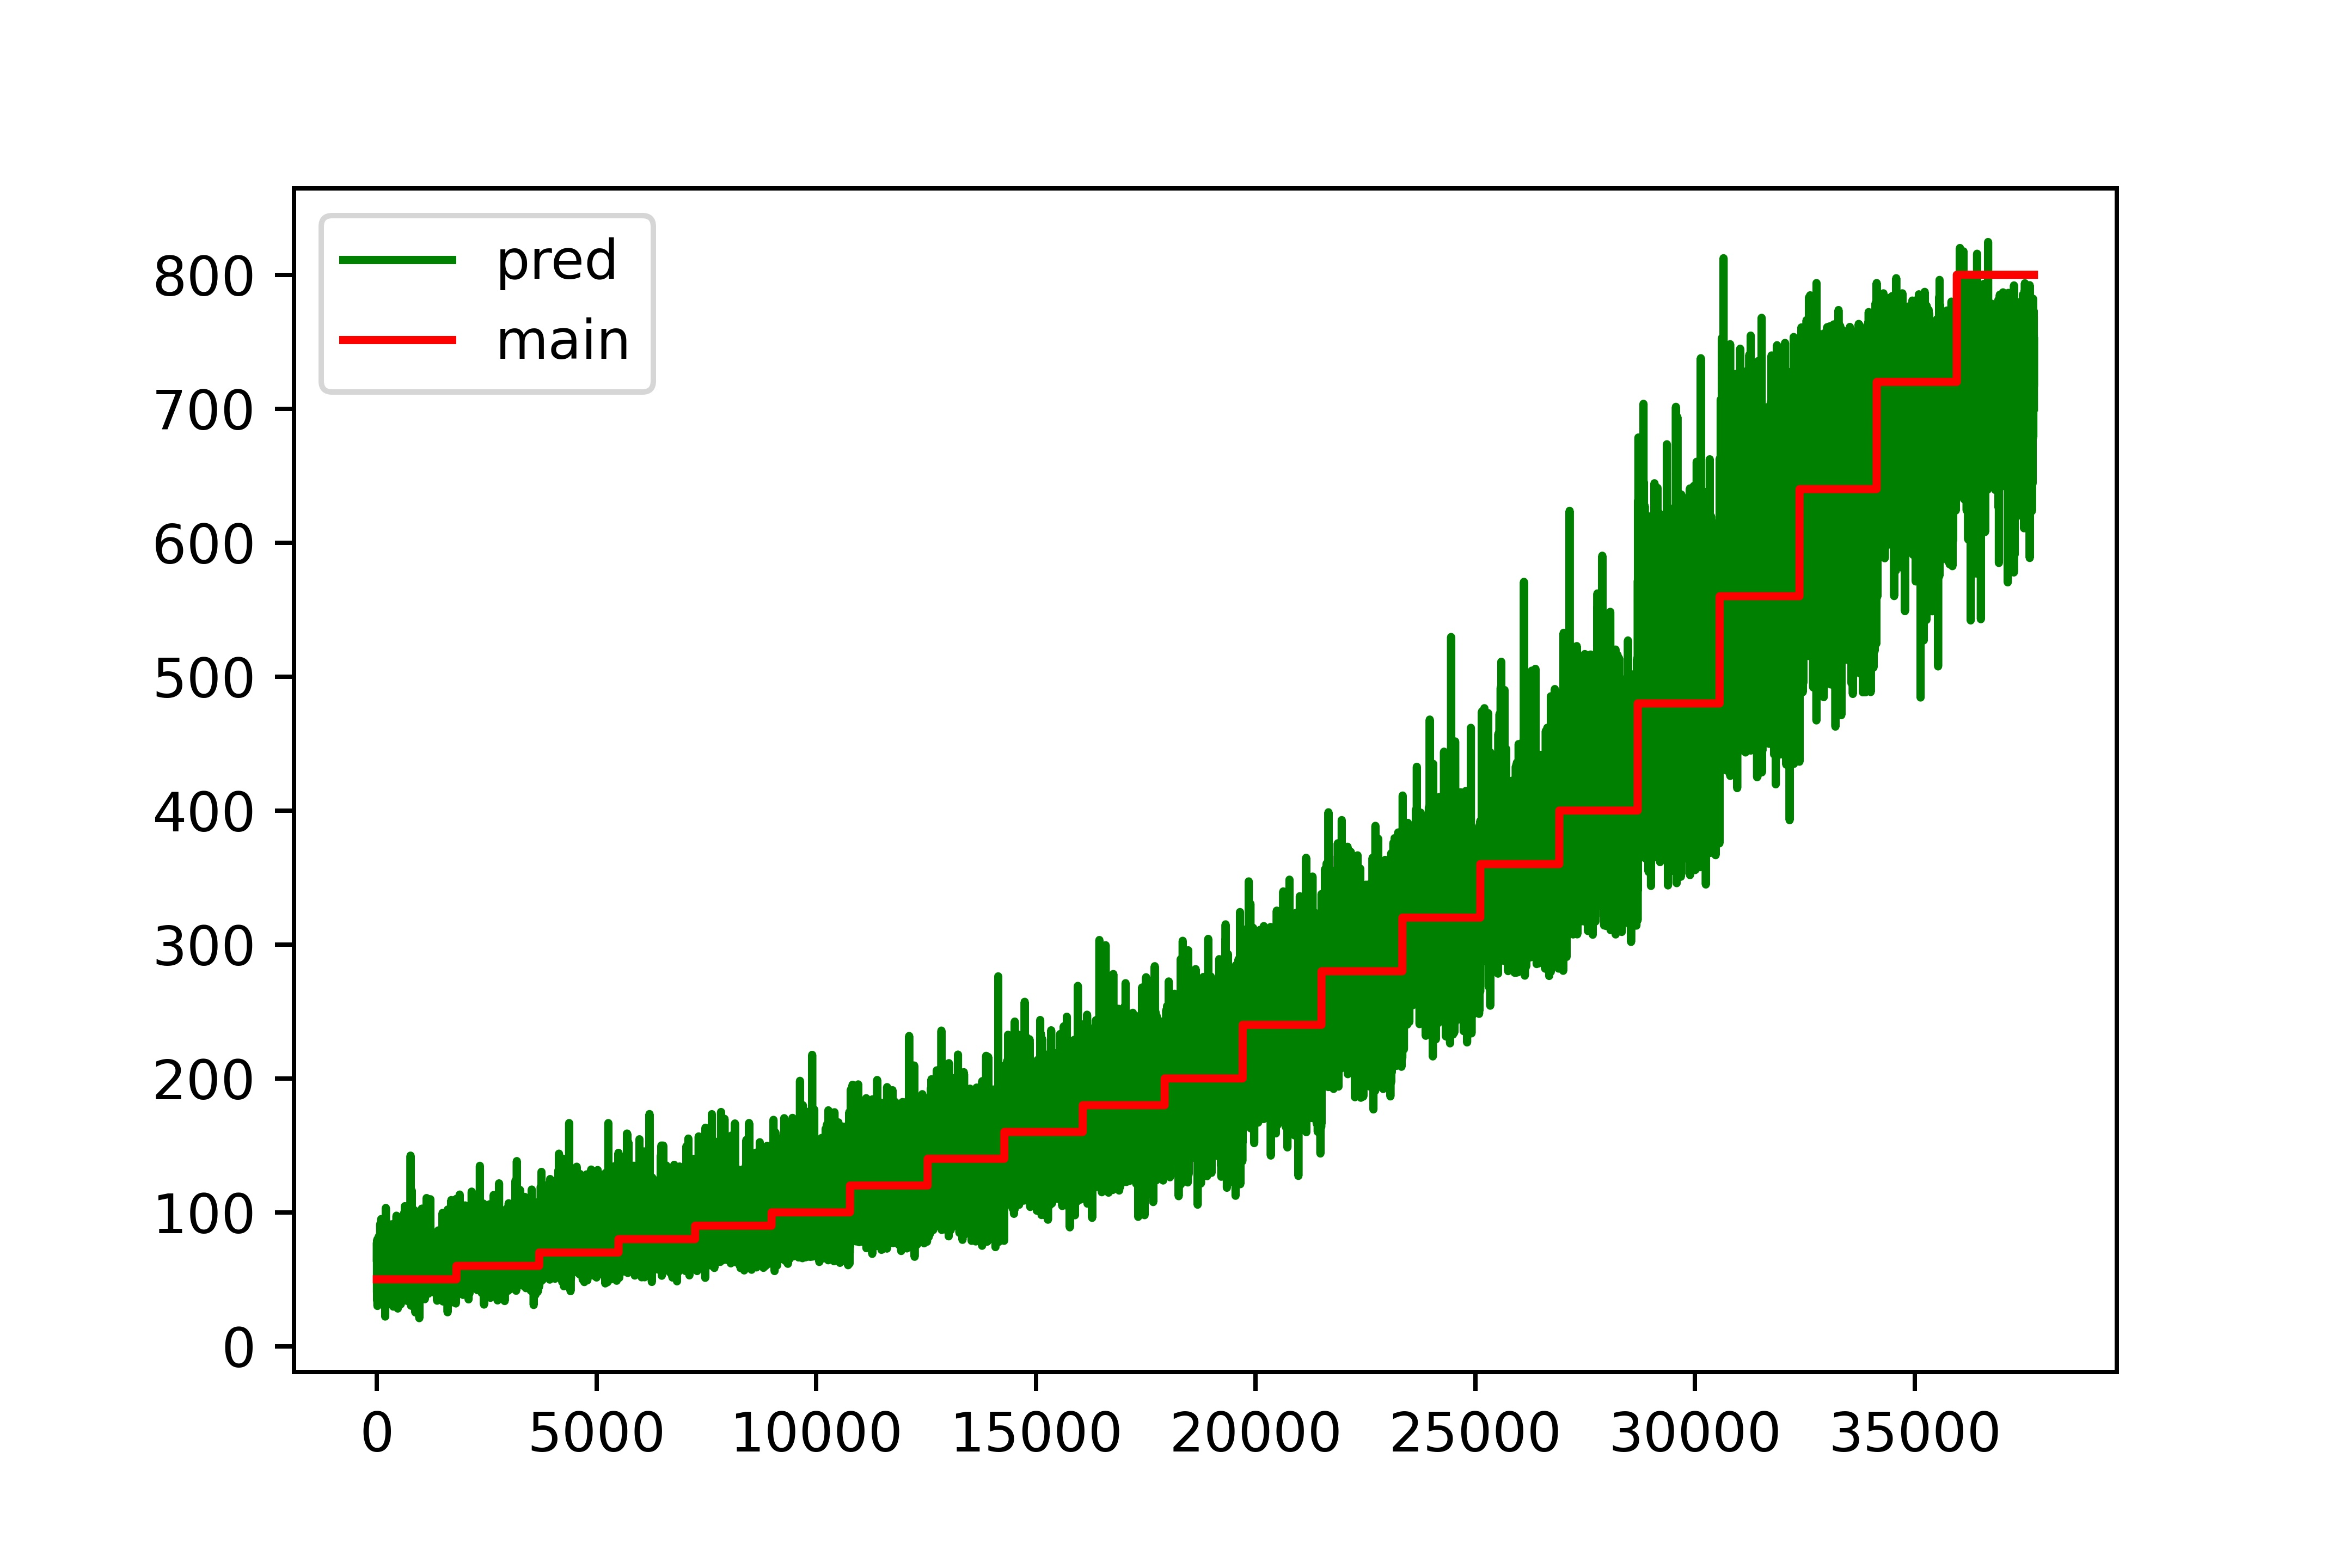
\includegraphics[width=12cm]{Images/adam_norm.jpg}
            \caption{Normalized result with ADAM optimizer. In Green, the predictions output. In red, the real values.}
            \label{fig:adam_norm}
        \end{figure}
        
        \begin{figure}[!h]
            \centering
            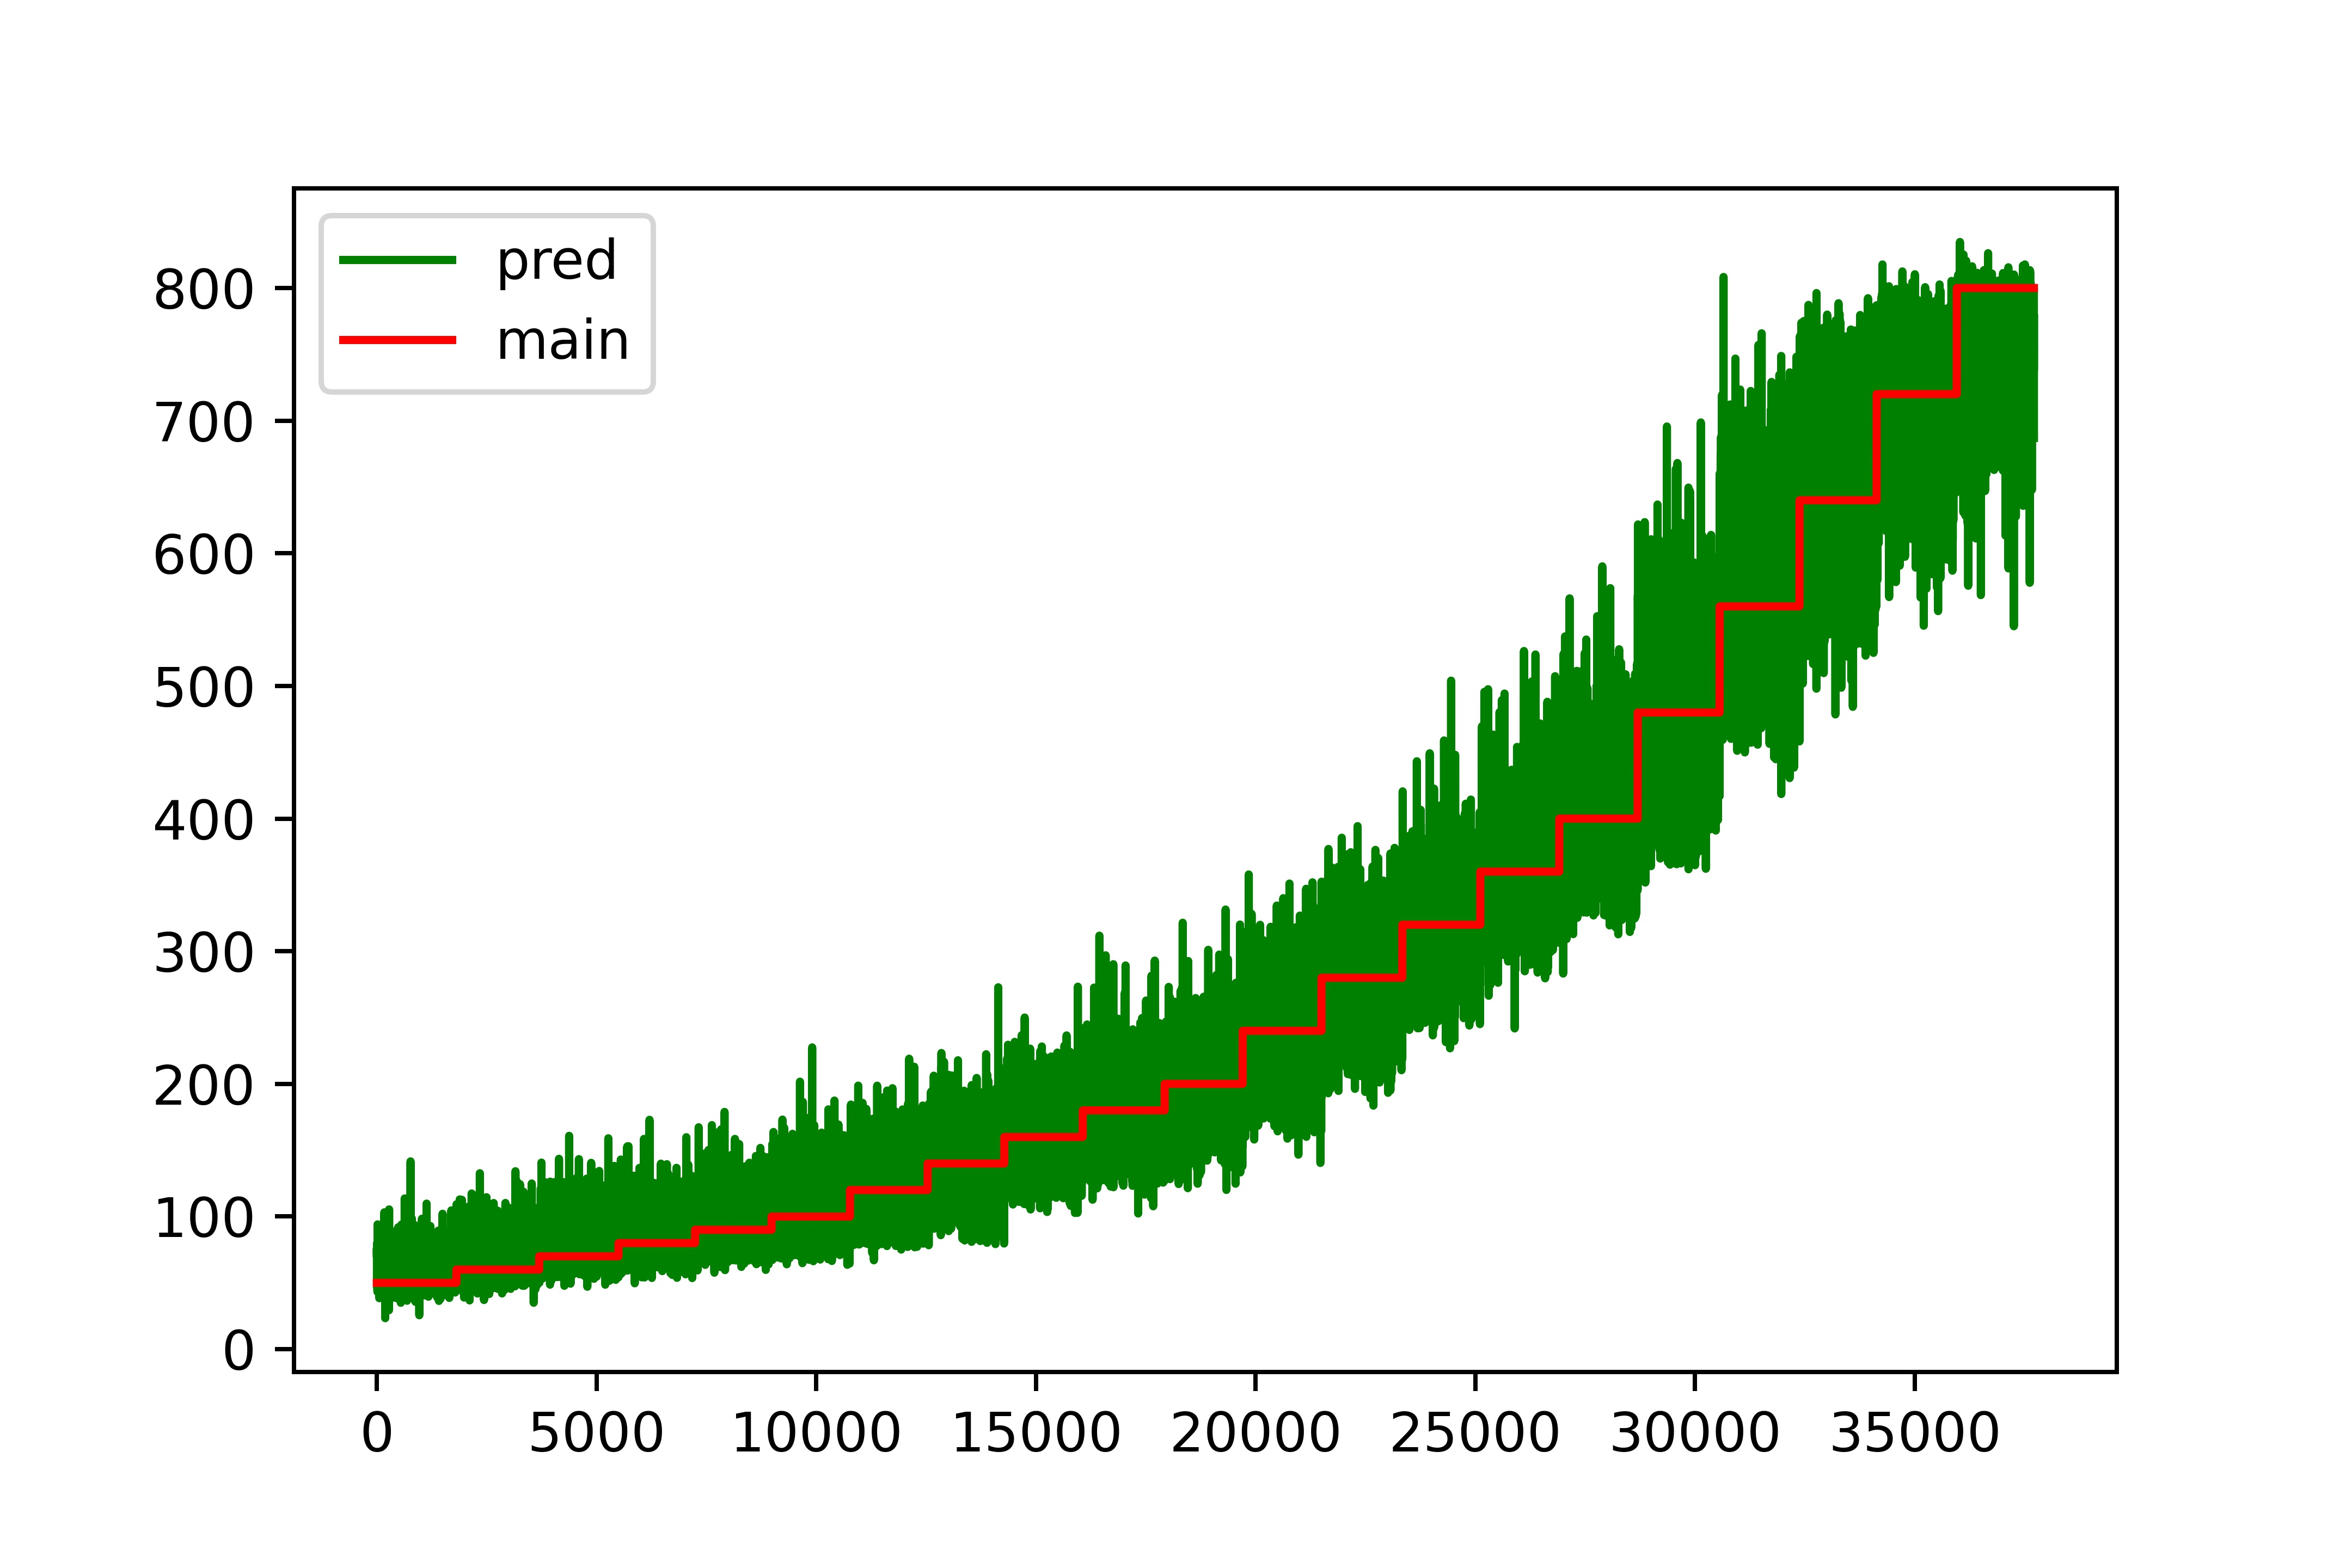
\includegraphics[width=12cm]{Images/plot_ada_norm.jpg}
            \caption {result with ADAGRAD optimizer. In Green, the predictions output. In red, the real values.}
            \label{fig:adagrad_norm}
        \end{figure}
    
    \subsection{Real Dataset}
    The real images were not used to train the network at any time, and its inference result for the first trial images can be seen in Fig. \ref{fig:cabedelo_pedras_prebias}. In red we can see the average height measured locally.
    For this set, the same optimizer used to get the best result for the synthetic bank was also employed, including the batch normalization. The accuracy in RMSE = 0.2928 and the loss = 0.0857, and the average inference for the actual height of 50cm = 71.95cm, and for 70cm = 125.47cm. 
    To fix the clear bias issue, a single subtraction was included at the output, as seen in \ref{fig:cabedelo_pedras}.
    
        \begin{figure}[!h]
            \centering
            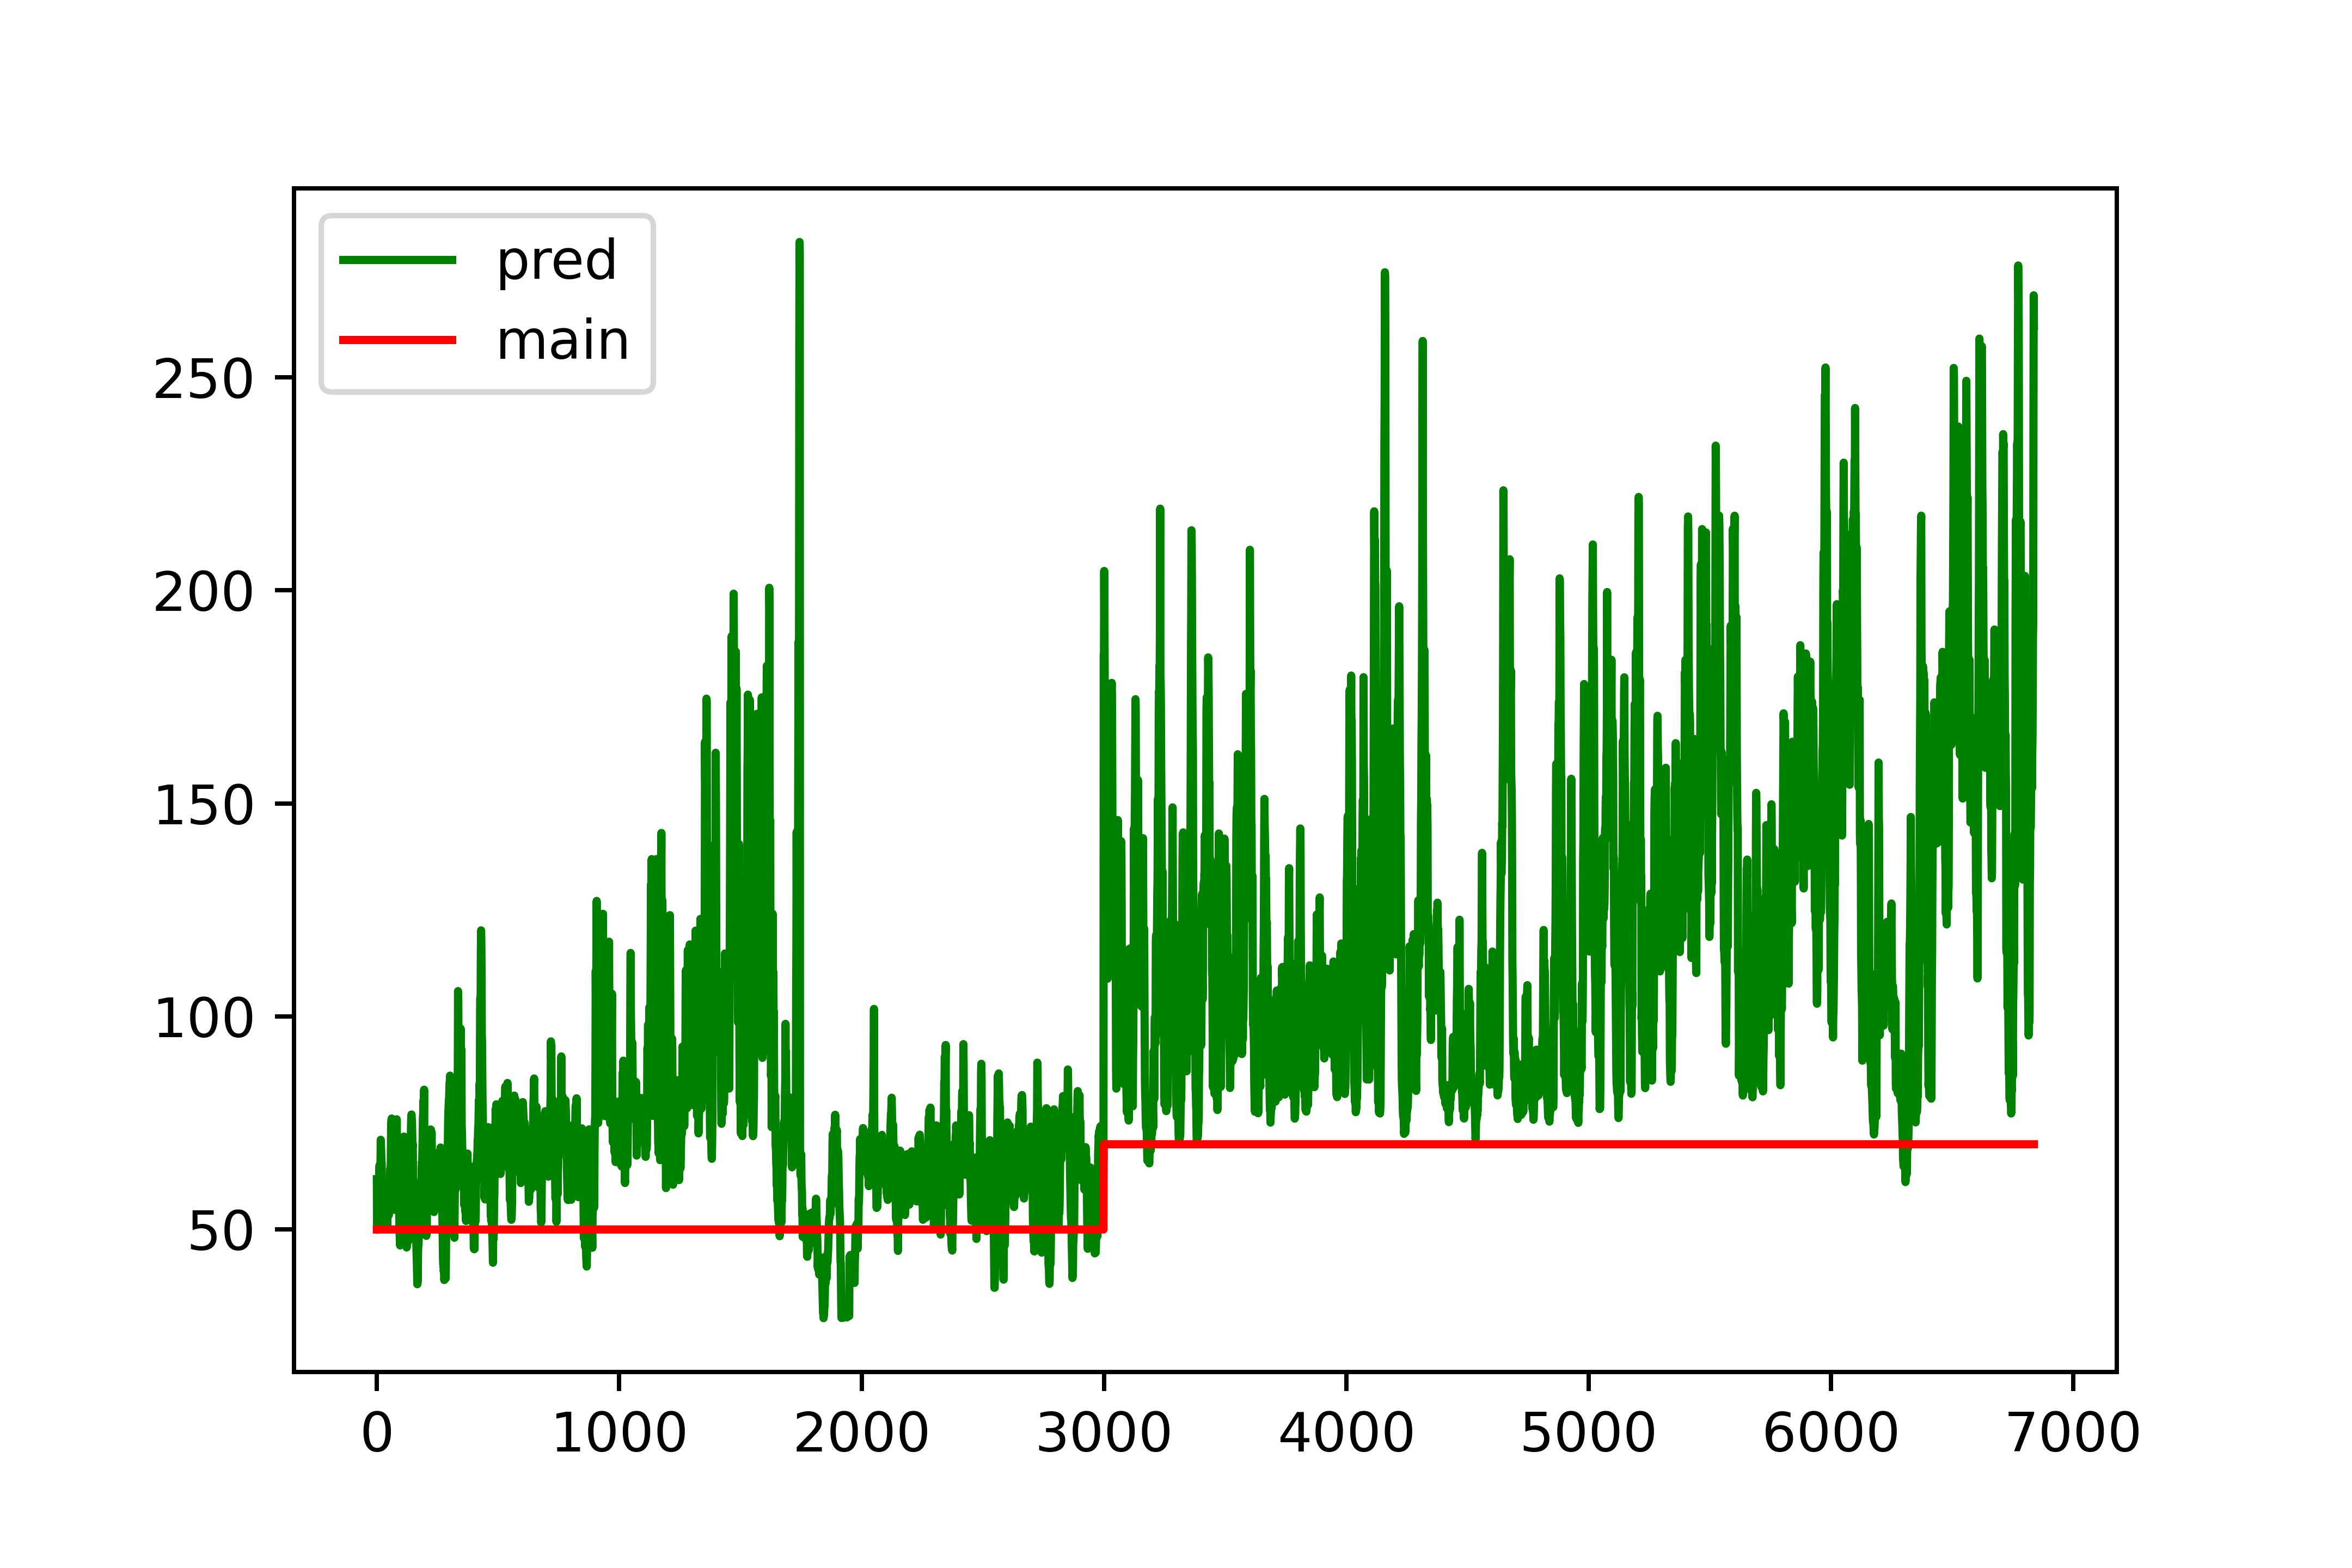
\includegraphics[width=12cm]{Images/cabedelo_pedras_prebias.jpg}
            \caption{Inference of the real data set with the final model. In Green, the predictions output. In red, the real values.}
            \label{fig:cabedelo_pedras_prebias}
        \end{figure}
        
        \begin{figure}[!h]
            \centering
            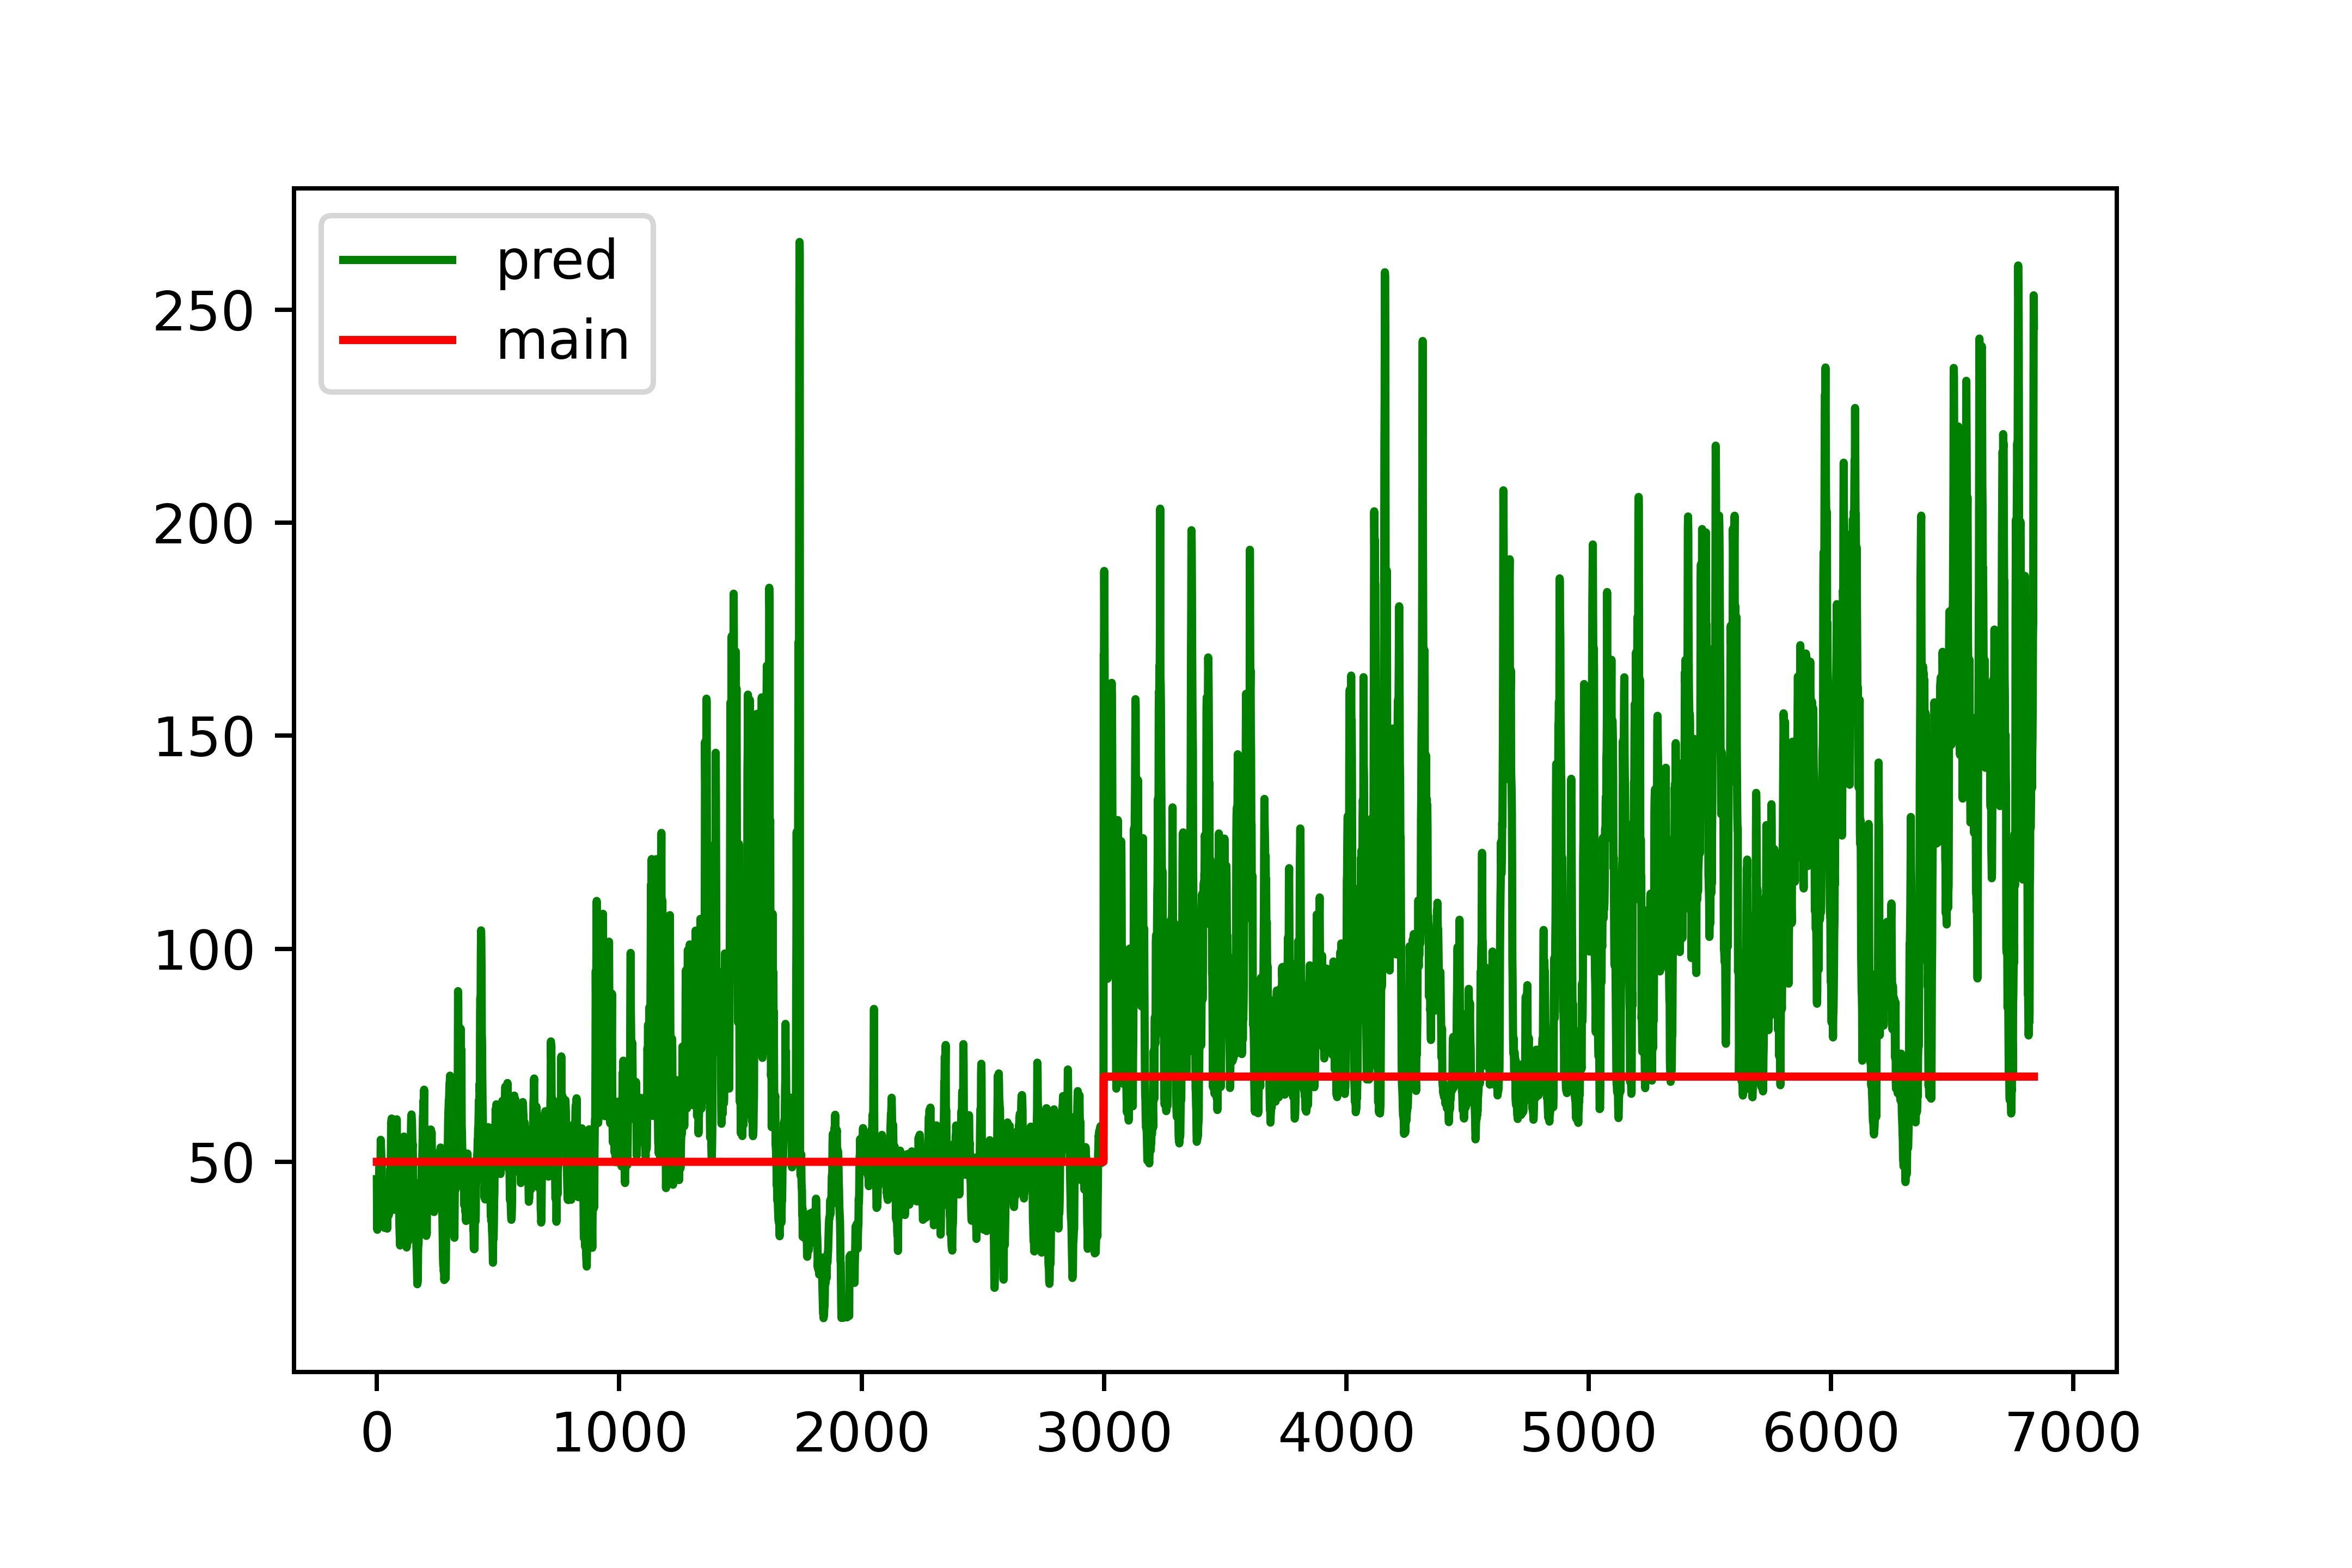
\includegraphics[width=12cm]{Images/cabedelo_pedras.jpg}
            \caption{Inference of the real data set with the final model after bias treatment. In Green, the predictions output. In red, the real values.}
            \label{fig:cabedelo_pedras}
        \end{figure}
    
    \subsection{Conclusion} 
    It was possible to verify, even with training on a synthetic bank, the recognition of different heights in real images with the trained network. This is better than initially expected, based on the fact that the whole image was rendered without any element found in the real environment, such as the presence of leaves, shadows, and stones.
    
    However, it was noticed an upward shift all over the predictions, which increases as there is also an increase in altitude.
    This phenomenon may be caused by:
    
    \begin{itemize}
        \item Error in the equipment itself; 
        \item Human inaccuracy in the camera operation;
        \item Bias inside the network, in concern of weights and filtering.
    \end{itemize}
    
    The first problem that can be repaired by using different methods, based on the availability of materials. On budget limitations, the already used pole can be adapted to a fixed pole solution, to adjust the camera height based on a height graduated ruler with clips. The ideal solution would be using a real drone to fly above water with human control, equipped with buoys on the frame foots to avoid sinking.
    
    %%%%FOTO DA BOIA%%%%